\documentclass[12pt]{article}
\usepackage[utf8]{inputenc}
\usepackage{amsfonts,amsmath,amssymb}
\usepackage[a4paper,left=20mm,right=20mm,top=20mm,bottom=20mm]{geometry}
\usepackage[loop,autoplay]{animate}
\usepackage{graphicx}
\usepackage{hyperref}
\usepackage{float}

\title{Assignment-4}
\author{MM21B046 }
\date{July 8 2022}

\begin{document}
	\maketitle
	{\huge\textbf{Wave equation}}\\
	\vspace{1cm}
	{\huge$$\frac{\partial^2u}{\partial t^2} = c^2\nabla^2u$$}
	\vspace{2cm}

\setlength{\parindent}{80pt}The (two-way) wave equati\textbf{on is a second-order linear partial differential equation for the description of waves or standing wave fields} — as they occur in classical physics — such as mechanical waves (e.g. water waves, sound waves and seismic waves) or electromagnetic waves (including light waves). It arises in fields like acoustics, electromagnetism, and fluid dynamics. A single wave propagating in a pre-defined direction can also be described with the one-way wave equation.

\vspace{2cm}
\begin{table}[H]
	\centering
	\caption{Table representing the symbols used and their description}
	\vspace{0.4cm}
	\def\arraystretch{1.5}
	\setlength{\tabcolsep}{50pt}
	\begin{tabular}{|l||c|}
		\hline
		Symbols used  &  Description of the symbols \\ \hline \hline
		$u$ & Amplitude of the wave\\
		\hline
		$t$ & time\\
		\hline
		$c$ & speed of the wave\\
		\hline
		$\nabla^2$ & Laplacian operator\\
		\hline
\end{tabular}
\end{table}


\begin{figure}[H]
		\caption{A 2D water wave}
	\begin{center}
		\frame{
		 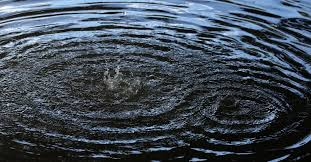
\includegraphics{images/waterwave.jpeg}}
	 \end{center}
	\vspace{2cm}
		\caption{\large A solution to 2D wave equation }
	\begin{center}
		 \frame{
		\animategraphics[trim=2 2cm 2 1.5cm,label=autoplay,loop,autoresume,controls={play,stop}]
		{12}{images/anim_}{4}{119}
		 }
	\end{center}{The above is a .gif.It can be viwed only in a pdf reader which can render vedios like okcular,evince,etc}
\end{figure}

\vspace{2cm}
\noindent{\large References:}\\[0.5cm]
\url{https://en.wikipedia.org/wiki/Wave_equation#:~:text=The%20(two%2Dway)%20wave,waves%20(including%20light%20waves).}

\end{document}
